\section{Benchmarks}

 We evaluate different approaches against the base MAPF encoding introduced in section~\ref{sec:background_mapf}. A witness approach is also evaluated. It consists of one random path per agent converted to a subgraph. Then applying the partial solver~\ref{lst:solver}. It aims to define a referential for the benchmark where shortest path are selected randomly. All used approaches in the benchmark are described in appendix tables~\ref{tbl:approach_ref_and_desc}.

At first, we introduce in Table \ref{tbl:nomenclature_approach} the nomenclature used to name the approaches:

\begin{table}[H]
    \centering
    \caption{Nomenclature of approaches names}
    \label{tbl:nomenclature_approach}
    \begin{tabular}{@{}c|c|c@{}}
    Step Name & Description & Identifier \\ \midrule
    \multirow{2}{*}{IPF} & No Additional path computed & \textbf{N} \\
     & Additional Path computed & \textbf{A} \\ \midrule
    \multirow{2}{*}{Path Elimination} & Simple threshold & \textbf{St} \\
     & Summed Heatmap & \textbf{Sh} \\ \midrule
    \multirow{2}{*}{\begin{tabular}[c]{@{}c@{}}Solving strategy\\ (can be both)\end{tabular}} & Pre-computed path & \textbf{Pc} \\
     & Subgraph & \textbf{Sg} \\ \midrule
    \multirow{2}{*}{Subgraph strategy} & Corridor & \textbf{C} \\
     & Diamond & \textbf{D}
    \end{tabular}
\end{table}

The benchmark were run on a Intel Core i7-4470 @ 3.60ghz with 16GiB of RAM with at most 5 minutes are allowed for each instances. The following values were used for various computations:

\begin{minipage}[H]{\linewidth}
\begin{itemize}
    \item 15 paths requested (30 paths if additional paths are requested)
    \item 1 paths retrieved for the killed agent for the subgraph approach
    \item A bias of 1 for the simple threshold
    \item 70\% of the highest summed heatmap paths are killed
    \item Corridors extension of size one
    \item Diamonds extension of size two  
\end{itemize}
\end{minipage} 


\subsection{Global result}

 Table~\ref{tbl:path_computation_time} shows; the identifier of the approach. The number of instance where it found a (partial) solution and last property outlined shows the average time required to compute a solution with a modified horizon (0 means that the horizon is equal to the makespan). Note that additional horizon is computed for Base MAPF for comparison purpose.


\begin{table}[H]
\begin{center}
\caption{Approaches: focus on average computation time}
\label{tbl:path_computation_time}
\begin{tabular}{@{}lllllll@{}}
\toprule
 \multicolumn{1}{c}{\multirow{2}{*}{Approach}} & \multirow{2}{*}{\# SAT} & \multicolumn{5}{c}{Average time (in sec)} \\ \cmidrule(l){3-7}  
\multicolumn{1}{c}{} &  & \multicolumn{1}{l|}{Horizon} & 0 & 1 & 3 & 5 \\ \midrule
NStPc & 41 & \cellcolor{lightgrey} & 86.3 & 110.8 & 136.7 & 164.3  \\
NStSgC & 44 & \cellcolor{lightgrey} & 14.7 & 29.4 & 38.0 & 47.0  \\
AShSg & 44 & \cellcolor{lightgrey} & 16.7 & 29.9 & 38.9 & 48.0  \\
AStPc & 39 & \cellcolor{lightgrey} & 128.2 & 152.6 & 178.7 & 206.0  \\
MAPF & 44 & \cellcolor{lightgrey} & 25.4 & 34.1 & 52.6 & 72.3  \\
NStSg & 44 & \cellcolor{lightgrey} & 14.5 & 29.1 & 37.8 & 46.6  \\
AStSgCD & 37 & \cellcolor{lightgrey} & 153.7 & 161.2 & 169.4 & 177.8  \\
NShSg & 44 & \cellcolor{lightgrey} & 14.3 & 28.5 & 37.4 & 46.6  \\
NShSgPc & 37 & \cellcolor{lightgrey} & 152.0 & 159.3 & 167.1 & 175.4  \\
AStSgPc & 37 & \cellcolor{lightgrey} & 153.4 & 160.9 & 169.1 & 177.5  \\
AStSg & 43 & \cellcolor{lightgrey} & 30.9 & 39.5 & 48.5 & 58.0  \\
Witness & 44 & \cellcolor{lightgrey} & 9.0 & 17.4 & 26.0 & 34.1  \\
NShSgPcCD & 40 & \cellcolor{lightgrey} & 92.7 & 100.4 & 108.7 & 117.6  \\
NStSgD & 44 & \cellcolor{lightgrey} & 14.6 & 29.5 & 38.1 & 47.1  \\
NShPc & 41 & \cellcolor{lightgrey} & 101.9 & 114.0 & 141.3 & 170.1  \\
NStSgPc & 38 & \cellcolor{lightgrey} & 131.5 & 138.6 & 146.2 & 154.5  \\
AShSgCD & 44 & \cellcolor{lightgrey} & 17.2 & 30.5 & 39.6 & 48.9  \\
NStSgCD & 44 & \cellcolor{lightgrey} & 14.7 & 29.6 & 38.3 & 47.2  \\
\end{tabular}
\end{center}
\end{table}


 Table \ref{tbl:path_computation_time} shows the disparity of efficiency among Plan Merging approaches. Particularly noteworthy is the \textbf{NShSg} approach, which stands out as the fastest among the tested methods. As expected, longer computation time is observed for approaches using additional paths in approaches like \textbf{AStSg}, \textbf{AStSgPc}, and \textbf{AStPc}.
It appears that precomputed paths approaches often times out or, more likely, produces unsat results. This can be attributed to way the paths are forced, described in our methodology, inevitably induces collision. Figure~\ref{fig:precomputed_path_conflict} illustrates a scenario where conflict(s) are inevitable using the pre-computed paths approach.
In all cases, the witness approach seems to be a faster approach while providing for each instances a solution.
\begin{figure}[H]
    \centering
    \caption{Inevitable conflict example for pre-computed path strategy}\label{fig:precomputed_path_conflict}
    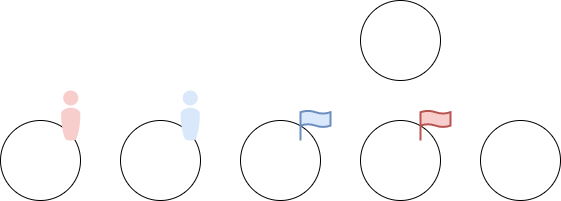
\includegraphics[width=\widthimg]{img/precomputed_path_conflict.drawio.png}
\end{figure}


With table~\ref{tbl:path_proportion}, we focus on the. "\# Fully solved instances" column refers to scenarios where all agents obtain a path. This table also presents the expected proportion of paths found given a modified horizon.

\begin{table}[H]
\begin{center}
\caption{Approaches: focus on solving path proportion}
\label{tbl:path_proportion}
\begin{tabular}{@{}lllllll@{}}
\toprule
 \multicolumn{1}{c}{\multirow{2}{*}{Approach}} & \multirow{2}{*}{\# fully solved} & \multicolumn{5}{c}{Expected \% agent with a path} \\ \cmidrule(l){3-7}  
\multicolumn{1}{c}{} &  & \multicolumn{1}{l|}{Horizon} & 0 & 1 & 3 & 5 \\ \midrule
NStPc & 24 & \cellcolor{lightgrey} & 86 & 87 & 88 & 90  \\
NStSgC & 37 & \cellcolor{lightgrey} & 97 & 97 & 98 & 98  \\
AShSg & 39 & \cellcolor{lightgrey} & 97 & 97 & 98 & 98  \\
AStPc & 22 & \cellcolor{lightgrey} & 80 & 80 & 82 & 83  \\
MAPF & 44 & \cellcolor{lightgrey} & 100 & 100 & 100 & 100  \\
NStSg & 37 & \cellcolor{lightgrey} & 97 & 97 & 98 & 98  \\
AStSgCD & 17 & \cellcolor{lightgrey} & 72 & 72 & 74 & 75  \\
NShSg & 37 & \cellcolor{lightgrey} & 96 & 96 & 97 & 98  \\
NShSgPc & 23 & \cellcolor{lightgrey} & 77 & 78 & 78 & 80  \\
AStSgPc & 17 & \cellcolor{lightgrey} & 72 & 72 & 74 & 75  \\
AStSg & 37 & \cellcolor{lightgrey} & 97 & 97 & 98 & 98  \\
Witness & 38 & \cellcolor{lightgrey} & 96 & 97 & 97 & 98  \\
NShSgPcCD & 21 & \cellcolor{lightgrey} & 83 & 83 & 84 & 85  \\
NStSgD & 37 & \cellcolor{lightgrey} & 97 & 97 & 98 & 98  \\
NShPc & 31 & \cellcolor{lightgrey} & 88 & 89 & 89 & 90  \\
NStSgPc & 15 & \cellcolor{lightgrey} & 75 & 76 & 77 & 78  \\
AShSgCD & 39 & \cellcolor{lightgrey} & 97 & 97 & 98 & 98  \\
NStSgCD & 37 & \cellcolor{lightgrey} & 97 & 97 & 98 & 98  \\
\end{tabular}
\end{center}
\end{table}


This table confirms result concluded with table~\ref{tbl:path_proportion}. Further emphasizing the effectiveness of the \textbf{NShSg} approach, which, among other, have the highest number of fully solved instances.  It also confirms that pre-computed paths approach do not perform well since it register the lowest score in terms of number of fully solved instances and in terms of expected proportion of agent with a path.
The data also indicates that combining Diamond and Corridor extensions does not appear to enhance the solving process. In fact, it even results in worse results compared to similar approaches without these extensions, as evidenced by \textbf{NShSgCD} compared to \textbf{NShSg} and \textbf{AStSgCD} compared to \textbf{AStSg}.
Furthermore, we can notice multiple approaches that are providing really high expected proportion of fully solved instance; \textbf{NStSg}, \textbf{NStSgCD}, \textbf{NStSgD}, \textbf{NStSgC} and \textbf{AStSg}.
Additionally, multiple approaches demonstrate high expected proportions of fully solved instances, including \textbf{NStSg}, \textbf{NStSgCD}, \textbf{NStSgD}, \textbf{NStSgC}, and \textbf{AStSg}.

It is noteworthy that increasing the horizon does not significantly impact the solving proportion. However, as expected, raising the horizon, always improve the ``expected \% agent with a path''.

From these tables, we selected the following approaches; \textbf{MAPF}, \textbf{Witness}, \textbf{AShSg}, \textbf{AStPc}, \textbf{AStSg} and \textbf{NShSg}.

\begin{figure}[H]
    \centering
    \caption{Cactus plot given selected approaches}\label{fig:cactus}
    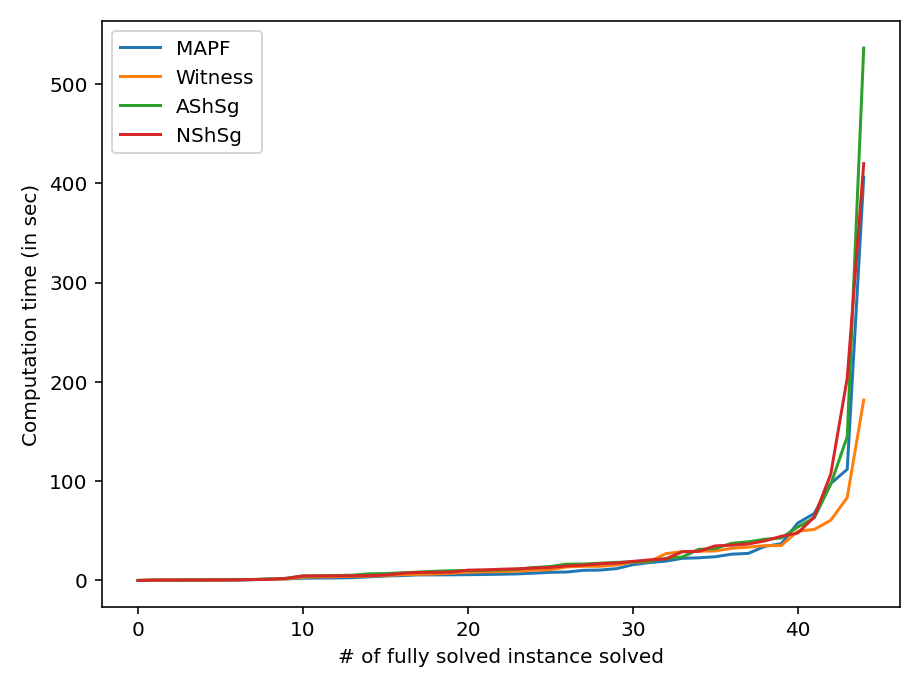
\includegraphics[width=\widthimg]{img/plt_cactus.png}
\end{figure}


The plot illustrated in Figure~\ref{fig:cactus}, shows the performance of some approaches. As computed for table~\ref{sec:pathselection}, to be considered as solved, an approach must find a path for all agents. 

Plan Merging approaches can provide a partial solution faster than the base MAPF encoding, but have worse result if we try to reach a complete solution. Given the great performance of the witness solver, it seems that the Path Selection processes we defined is not efficient. It however shows that separating MAPF in two steps improves the computation time. With a better and smarter IPF, we possibly can provide even better results.


\subsubsection{Detailed performance}

From the best approach \textbf{NShSg} outlined by the previous result, we provide in Table~\ref{tbl:approach_decomposition}, the total time and the proportion of each steps composing the approach.

\begin{table}[]
    \centering
    \caption{Approach Decomposition}\label{tbl:approach_decomposition}
    \begin{tabular}{@{}llllll@{}}
    \toprule
    \multicolumn{1}{l|}{\multirow{2}{*}{Step Name}} & \multicolumn{3}{c|}{Total time} & \multicolumn{2}{c}{\% of the process} \\ \cmidrule(l){2-6}  
    \multicolumn{1}{l|}{} & \multicolumn{1}{l|}{Id.} & \multicolumn{1}{c}{NShSg} & \multicolumn{1}{c|}{Witness} & \multicolumn{1}{c}{AShSg} & Witness \\ \midrule
    IPF & \cellcolor{lightgrey} & 49 & 41  &7\% &10\%  \\
    Heatmaps Computation & \cellcolor{lightgrey} & 14 &  - &2\% & - \\
    Summed Heatmap per Path & \cellcolor{lightgrey} & 0 &  - &0\% & - \\
    Path Elimination & \cellcolor{lightgrey} & 7 &  - &1\% & - \\
    Path Selection & \cellcolor{lightgrey} & 8 & 1  &1\% &0\%  \\
    Partial Solving & \cellcolor{lightgrey} & 551 & 352  &87\% &89\%  \\
    \end{tabular}
    \end{table}

    
The table illustrates the time distribution across different steps of the approach. While generating initial paths is relatively efficient, the process of finding partial solutions is a significant portion of the computation time. These insights tells us that  \textbf{partial solving} requires the most an optimization. However, this step depends on all previous steps and on the solver itself. Another possible optimization track is the IPF step which could be improved with a faster programming language. On the other hand the \textbf{witness} approach shows us that one random path is enough to have really good result. 



